%\subsection{Portfolio f\"ur Evaluation Method und Property Instance (Gr\"o\ss{}e entspricht der Anzahl)}
%\begin{figure}
\begin{center}
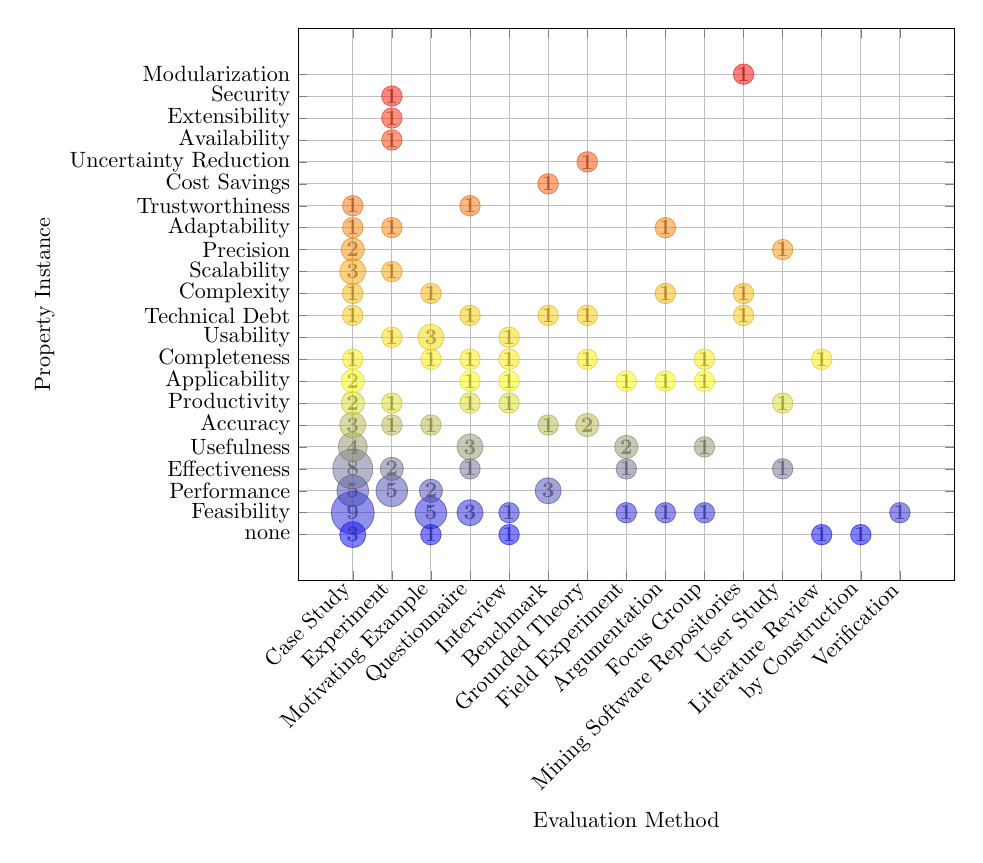
\begin{tikzpicture}[scale=.8]
\begin{axis}[scatter,
    width=.99\linewidth,
    cycle multi list=Spectral,
    every axis plot/.append style={draw, fill, fill opacity=0.5},
    scatter src=y,
    nodes near coords style={color=black,font=\small},
    %enlargelimits=0.15,
    x tick label style={rotate=45,anchor=east},
    xtick={0,1,2,3,4,5,6,7,8,9,10,11,12,13,14}, xticklabels={Case Study,Experiment,Motivating Example,Questionnaire,Interview,Benchmark,Grounded Theory,Field Experiment,Argumentation,Focus Group,Mining Software Repositories,User Study,Literature Review,by Construction,Verification},
    xlabel={Evaluation Method},
    ytick={0,1,2,3,4,5,6,7,8,9,10,11,12,13,14,15,16,17,18,19,20,21}, yticklabels={none,Feasibility,Performance,Effectiveness,Usefulness,Accuracy,Productivity,Applicability,Completeness,Usability,Technical Debt,Complexity,Scalability,Precision,Adaptability,Trustworthiness,Cost Savings,Uncertainty Reduction,Availability,Extensibility,Security,Modularization},
    ylabel={Property Instance},
    grid=both
]

\addplot[mark size=5.890,opacity=0.5,text=black] coordinates { (0,0) } node[text=black,font=\bfseries] {3};
\addplot[mark size=9.669,opacity=0.5,text=black] coordinates { (0,1) } node[text=black,font=\bfseries] {9};
\addplot[mark size=7.150,opacity=0.5,text=black] coordinates { (0,2) } node[text=black,font=\bfseries] {5};
\addplot[mark size=9.039,opacity=0.5,text=black] coordinates { (0,3) } node[text=black,font=\bfseries] {8};
\addplot[mark size=6.520,opacity=0.5,text=black] coordinates { (0,4) } node[text=black,font=\bfseries] {4};
\addplot[mark size=5.890,opacity=0.5,text=black] coordinates { (0,5) } node[text=black,font=\bfseries] {3};
\addplot[mark size=5.260,opacity=0.5,text=black] coordinates { (0,6) } node[text=black,font=\bfseries] {2};
\addplot[mark size=5.260,opacity=0.5,text=black] coordinates { (0,7) } node[text=black,font=\bfseries] {2};
\addplot[mark size=4.630,opacity=0.5,text=black] coordinates { (0,8) } node[text=black,font=\bfseries] {1};
\addplot[mark size=4.630,opacity=0.5,text=black] coordinates { (0,10) } node[text=black,font=\bfseries] {1};
\addplot[mark size=4.630,opacity=0.5,text=black] coordinates { (0,11) } node[text=black,font=\bfseries] {1};
\addplot[mark size=5.890,opacity=0.5,text=black] coordinates { (0,12) } node[text=black,font=\bfseries] {3};
\addplot[mark size=5.260,opacity=0.5,text=black] coordinates { (0,13) } node[text=black,font=\bfseries] {2};
\addplot[mark size=4.630,opacity=0.5,text=black] coordinates { (0,14) } node[text=black,font=\bfseries] {1};
\addplot[mark size=4.630,opacity=0.5,text=black] coordinates { (0,15) } node[text=black,font=\bfseries] {1};
\addplot[mark size=7.150,opacity=0.5,text=black] coordinates { (1,2) } node[text=black,font=\bfseries] {5};
\addplot[mark size=5.260,opacity=0.5,text=black] coordinates { (1,3) } node[text=black,font=\bfseries] {2};
\addplot[mark size=4.630,opacity=0.5,text=black] coordinates { (1,5) } node[text=black,font=\bfseries] {1};
\addplot[mark size=4.630,opacity=0.5,text=black] coordinates { (1,6) } node[text=black,font=\bfseries] {1};
\addplot[mark size=4.630,opacity=0.5,text=black] coordinates { (1,9) } node[text=black,font=\bfseries] {1};
\addplot[mark size=4.630,opacity=0.5,text=black] coordinates { (1,12) } node[text=black,font=\bfseries] {1};
\addplot[mark size=4.630,opacity=0.5,text=black] coordinates { (1,14) } node[text=black,font=\bfseries] {1};
\addplot[mark size=4.630,opacity=0.5,text=black] coordinates { (1,18) } node[text=black,font=\bfseries] {1};
\addplot[mark size=4.630,opacity=0.5,text=black] coordinates { (1,19) } node[text=black,font=\bfseries] {1};
\addplot[mark size=4.630,opacity=0.5,text=black] coordinates { (1,20) } node[text=black,font=\bfseries] {1};
\addplot[mark size=4.630,opacity=0.5,text=black] coordinates { (2,0) } node[text=black,font=\bfseries] {1};
\addplot[mark size=7.150,opacity=0.5,text=black] coordinates { (2,1) } node[text=black,font=\bfseries] {5};
\addplot[mark size=5.260,opacity=0.5,text=black] coordinates { (2,2) } node[text=black,font=\bfseries] {2};
\addplot[mark size=4.630,opacity=0.5,text=black] coordinates { (2,5) } node[text=black,font=\bfseries] {1};
\addplot[mark size=4.630,opacity=0.5,text=black] coordinates { (2,8) } node[text=black,font=\bfseries] {1};
\addplot[mark size=5.890,opacity=0.5,text=black] coordinates { (2,9) } node[text=black,font=\bfseries] {3};
\addplot[mark size=4.630,opacity=0.5,text=black] coordinates { (2,11) } node[text=black,font=\bfseries] {1};
\addplot[mark size=5.890,opacity=0.5,text=black] coordinates { (3,1) } node[text=black,font=\bfseries] {3};
\addplot[mark size=4.630,opacity=0.5,text=black] coordinates { (3,3) } node[text=black,font=\bfseries] {1};
\addplot[mark size=5.890,opacity=0.5,text=black] coordinates { (3,4) } node[text=black,font=\bfseries] {3};
\addplot[mark size=4.630,opacity=0.5,text=black] coordinates { (3,6) } node[text=black,font=\bfseries] {1};
\addplot[mark size=4.630,opacity=0.5,text=black] coordinates { (3,7) } node[text=black,font=\bfseries] {1};
\addplot[mark size=4.630,opacity=0.5,text=black] coordinates { (3,8) } node[text=black,font=\bfseries] {1};
\addplot[mark size=4.630,opacity=0.5,text=black] coordinates { (3,10) } node[text=black,font=\bfseries] {1};
\addplot[mark size=4.630,opacity=0.5,text=black] coordinates { (3,15) } node[text=black,font=\bfseries] {1};
\addplot[mark size=4.630,opacity=0.5,text=black] coordinates { (4,0) } node[text=black,font=\bfseries] {1};
\addplot[mark size=4.630,opacity=0.5,text=black] coordinates { (4,1) } node[text=black,font=\bfseries] {1};
\addplot[mark size=4.630,opacity=0.5,text=black] coordinates { (4,6) } node[text=black,font=\bfseries] {1};
\addplot[mark size=4.630,opacity=0.5,text=black] coordinates { (4,7) } node[text=black,font=\bfseries] {1};
\addplot[mark size=4.630,opacity=0.5,text=black] coordinates { (4,8) } node[text=black,font=\bfseries] {1};
\addplot[mark size=4.630,opacity=0.5,text=black] coordinates { (4,9) } node[text=black,font=\bfseries] {1};
\addplot[mark size=5.890,opacity=0.5,text=black] coordinates { (5,2) } node[text=black,font=\bfseries] {3};
\addplot[mark size=4.630,opacity=0.5,text=black] coordinates { (5,5) } node[text=black,font=\bfseries] {1};
\addplot[mark size=4.630,opacity=0.5,text=black] coordinates { (5,10) } node[text=black,font=\bfseries] {1};
\addplot[mark size=4.630,opacity=0.5,text=black] coordinates { (5,16) } node[text=black,font=\bfseries] {1};
\addplot[mark size=5.260,opacity=0.5,text=black] coordinates { (6,5) } node[text=black,font=\bfseries] {2};
\addplot[mark size=4.630,opacity=0.5,text=black] coordinates { (6,8) } node[text=black,font=\bfseries] {1};
\addplot[mark size=4.630,opacity=0.5,text=black] coordinates { (6,10) } node[text=black,font=\bfseries] {1};
\addplot[mark size=4.630,opacity=0.5,text=black] coordinates { (6,17) } node[text=black,font=\bfseries] {1};
\addplot[mark size=4.630,opacity=0.5,text=black] coordinates { (7,1) } node[text=black,font=\bfseries] {1};
\addplot[mark size=4.630,opacity=0.5,text=black] coordinates { (7,3) } node[text=black,font=\bfseries] {1};
\addplot[mark size=5.260,opacity=0.5,text=black] coordinates { (7,4) } node[text=black,font=\bfseries] {2};
\addplot[mark size=4.630,opacity=0.5,text=black] coordinates { (7,7) } node[text=black,font=\bfseries] {1};
\addplot[mark size=4.630,opacity=0.5,text=black] coordinates { (8,1) } node[text=black,font=\bfseries] {1};
\addplot[mark size=4.630,opacity=0.5,text=black] coordinates { (8,7) } node[text=black,font=\bfseries] {1};
\addplot[mark size=4.630,opacity=0.5,text=black] coordinates { (8,11) } node[text=black,font=\bfseries] {1};
\addplot[mark size=4.630,opacity=0.5,text=black] coordinates { (8,14) } node[text=black,font=\bfseries] {1};
\addplot[mark size=4.630,opacity=0.5,text=black] coordinates { (9,1) } node[text=black,font=\bfseries] {1};
\addplot[mark size=4.630,opacity=0.5,text=black] coordinates { (9,4) } node[text=black,font=\bfseries] {1};
\addplot[mark size=4.630,opacity=0.5,text=black] coordinates { (9,7) } node[text=black,font=\bfseries] {1};
\addplot[mark size=4.630,opacity=0.5,text=black] coordinates { (9,8) } node[text=black,font=\bfseries] {1};
\addplot[mark size=4.630,opacity=0.5,text=black] coordinates { (10,10) } node[text=black,font=\bfseries] {1};
\addplot[mark size=4.630,opacity=0.5,text=black] coordinates { (10,11) } node[text=black,font=\bfseries] {1};
\addplot[mark size=4.630,opacity=0.5,text=black] coordinates { (10,21) } node[text=black,font=\bfseries] {1};
\addplot[mark size=4.630,opacity=0.5,text=black] coordinates { (11,3) } node[text=black,font=\bfseries] {1};
\addplot[mark size=4.630,opacity=0.5,text=black] coordinates { (11,6) } node[text=black,font=\bfseries] {1};
\addplot[mark size=4.630,opacity=0.5,text=black] coordinates { (11,13) } node[text=black,font=\bfseries] {1};
\addplot[mark size=4.630,opacity=0.5,text=black] coordinates { (12,0) } node[text=black,font=\bfseries] {1};
\addplot[mark size=4.630,opacity=0.5,text=black] coordinates { (12,8) } node[text=black,font=\bfseries] {1};
\addplot[mark size=4.630,opacity=0.5,text=black] coordinates { (13,0) } node[text=black,font=\bfseries] {1};
\addplot[mark size=4.630,opacity=0.5,text=black] coordinates { (14,1) } node[text=black,font=\bfseries] {1};


\end{axis}
\end{tikzpicture}
\end{center}
%\caption{Portfolio f\"ur Evaluation Method und Property Instance (Gr\"o\ss{}e entspricht der Anzahl)}\label{fig:port_evaluationmethod_propertyinstance}
%\end{figure}

